\documentclass[11pt]{cernrep}
\usepackage{graphicx,epsfig}
\bibliographystyle{lesHouches}
\begin{document}
 
\section{Irreducible backgrounds and measurement uncertainties  \protect\footnote{Section
    coordinators: Jonathan M. Butterworth, Frank Krauss } $^{,}$ \protect\footnote{Vitaliano Ciulli, Paolo
  Francavilla, Vasilis Konstantinides, Piergiulio Lenzi, Carlo Pandini, Luca Perrozzi, Lorenzo Russo, Umit
  Utku, Lorenzo Viliani, Ben Waugh} $^{,}$ \protect\footnote{VC and LR
  acknowledge support by MIUR Italy under Grant Agreement 2012Z23ERZ of PRIN 2012}}

%$^1$Department of Physics and Astronomy, University College London,\\ 
%$^2$IPPP, Department of Physics, Durham University}

%\begin{abstract}
%A brief discussion and study of the treatment of irreducible backgrounds in $W+b$-jets and $WWbb$ production is presented.
%\end{abstract}

\subsection{Introduction}
\label{sec:intro}

The general principle of minimising the model-dependence of results from particle colliders by making measurements of 
well-defined final states in fiducial regions is by now widely accepted, and implemented by the LHC collaborations. 
The fiducial regions are designed to reflect  the acceptance of the detectors and data-selection. 
The final states are defined in terms of stable, or quasi-stable,
particles. Increasingly impressive theoretical calculations are able to implement the appropriate kinematic cuts, and
modulo some uncertainty associated with soft physics (for example hadronisation), can predict precisely what 
is actually being measured, without the need for additional assumptions or extrapolations into unmeasured regions of 
phase space.

This represents great progress. One area, however, where the principle of defining a measurement in terms of the final state
is not so widely implemented, is in the consideration of background processes and their subtraction. 
Often backgrounds are subtracted using a mixture of theoretical and data-driven techniques, 
even though in some cases the backgrounds are strictly speaking ``irreducible'', in that they produce final states 
identical to the ``signal'' final state (even in a perfect detector) and thus should be added to the signal 
at the amplitude, rather than cross-section, level. These subtractions are also often carried out before, or intermingled with, 
the unfolding and correction for detector effects such as efficiency and resolution, and thus are impossible to
undo or redo after the fact. 

In practice, the uncertainty introduced by such subtractions is often insignificant compared to other uncertainties in the measurements, 
for example because the kinematic overlap
is in fact small and interference terms are negligible. Nevertheless, in some processes, and as precision of both experiment
and theory increase, such considerations can become important. In this contribution we highlight some such cases in an attempt 
to raise awareness of the issues for future studies. 

\subsection{Single top and $W+b$ production}

An example of a final state in which two contributions are often treated as distinct processes is the measurement of a 
leptonically-decaying $W$ boson (that is, charged lepton plus missing transverse energy) in association with a $b$-tagged hadronic jet. 
The publication of the ATLAS analysis of 7~TeV collision data\cite{Aad:2013vka} contains a measurement of the fiducial $W+b$-jet 
cross section both with and without the subtraction of the single-top contribution to the identical final state. Both
versions are available in HEPDATA~\cite{hepdata} and Rivet~\cite{Buckley:2010ar}\footnote{The Rivet analysis was modified to add the histograms 
for the unsubtracted data.}. 
The unsubtracted version is shown in Fig.~\ref{fig:wb}, and the subtracted version in Fig.~\ref{fig:notop}. 

\begin{figure}
\begin{center}
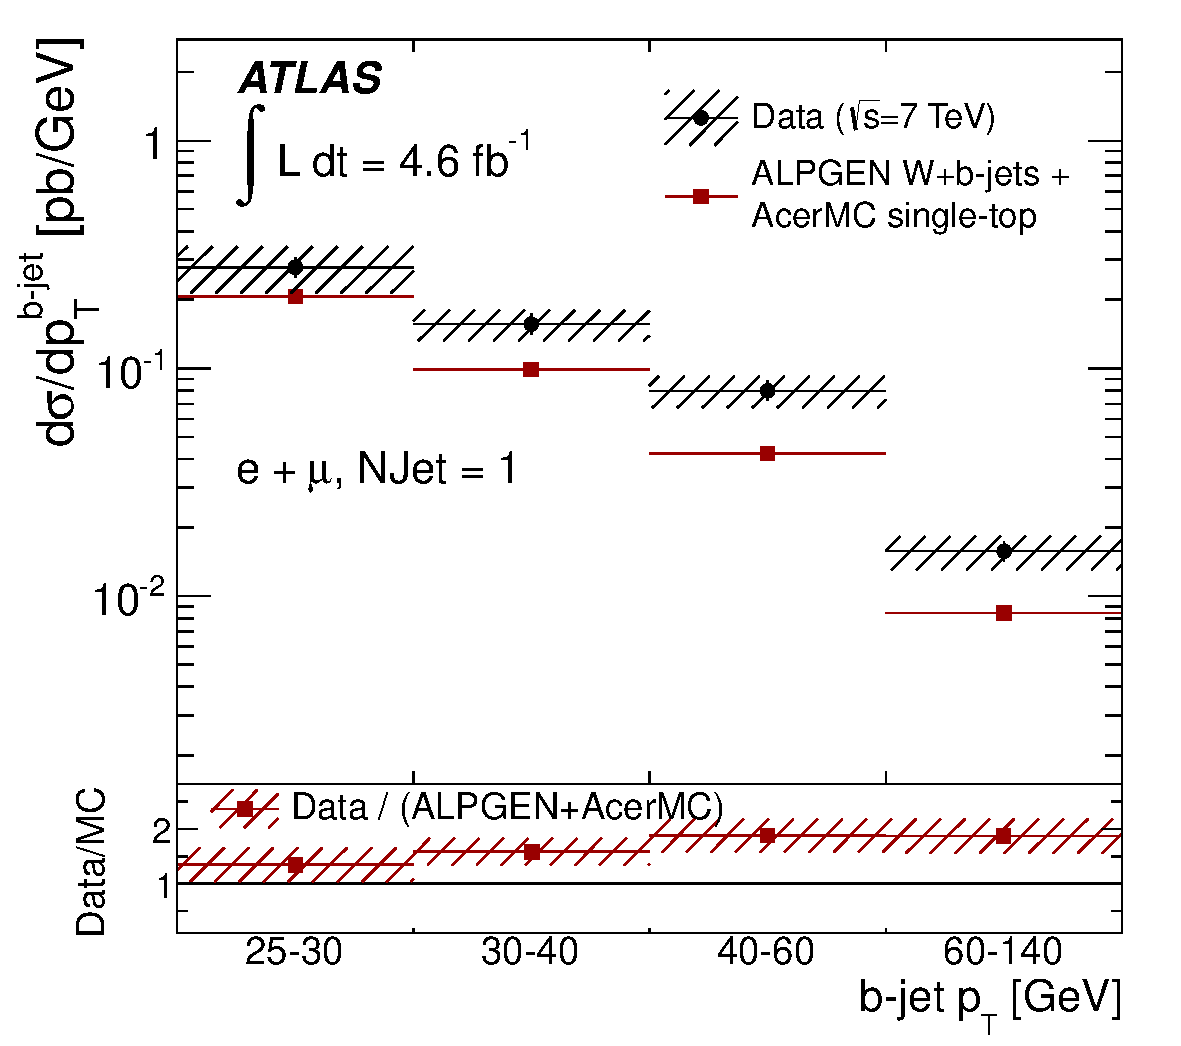
\includegraphics[width=0.48\textwidth]{fig_09a.pdf}
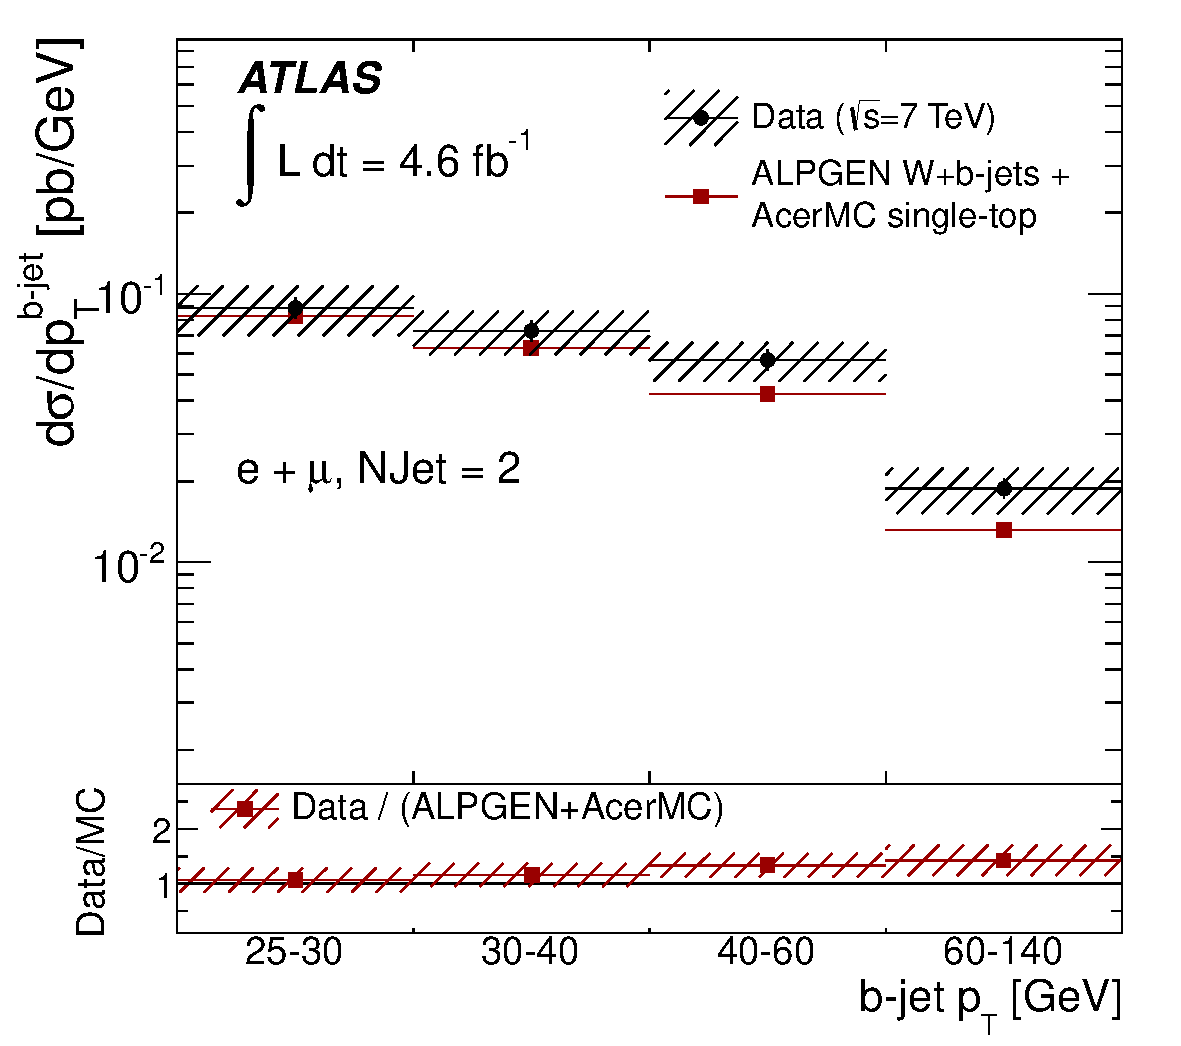
\includegraphics[width=0.48\textwidth]{fig_09b.pdf}
\caption{\label{fig:wb}
Measured differential $W+b$-jets cross-section without single-top subtraction as a function of the transverse momentum of the $b$-jet, in the 
case where the $b$-jet is the only jet in the fiducial region (left) or when there is an additional jet (right). 
%The cross sections are obtained by combining the electron and muon channels. 
The measurements are compared to the sum of separate $W+b$-jets and single-top predictions 
obtained using ALPGEN interfaced to HERWIG and JIMMY and scaled by a NNLO inclusive $W$ normalization factor, and ACERMC interfaced to PYTHIA and scaled to a 
NLO single-top cross-section. 
The ratios between measured and predicted cross-sections are also shown. From~\protect\cite{Aad:2013vka}.}
\end{center}
\end{figure}

\begin{figure}
\centering
	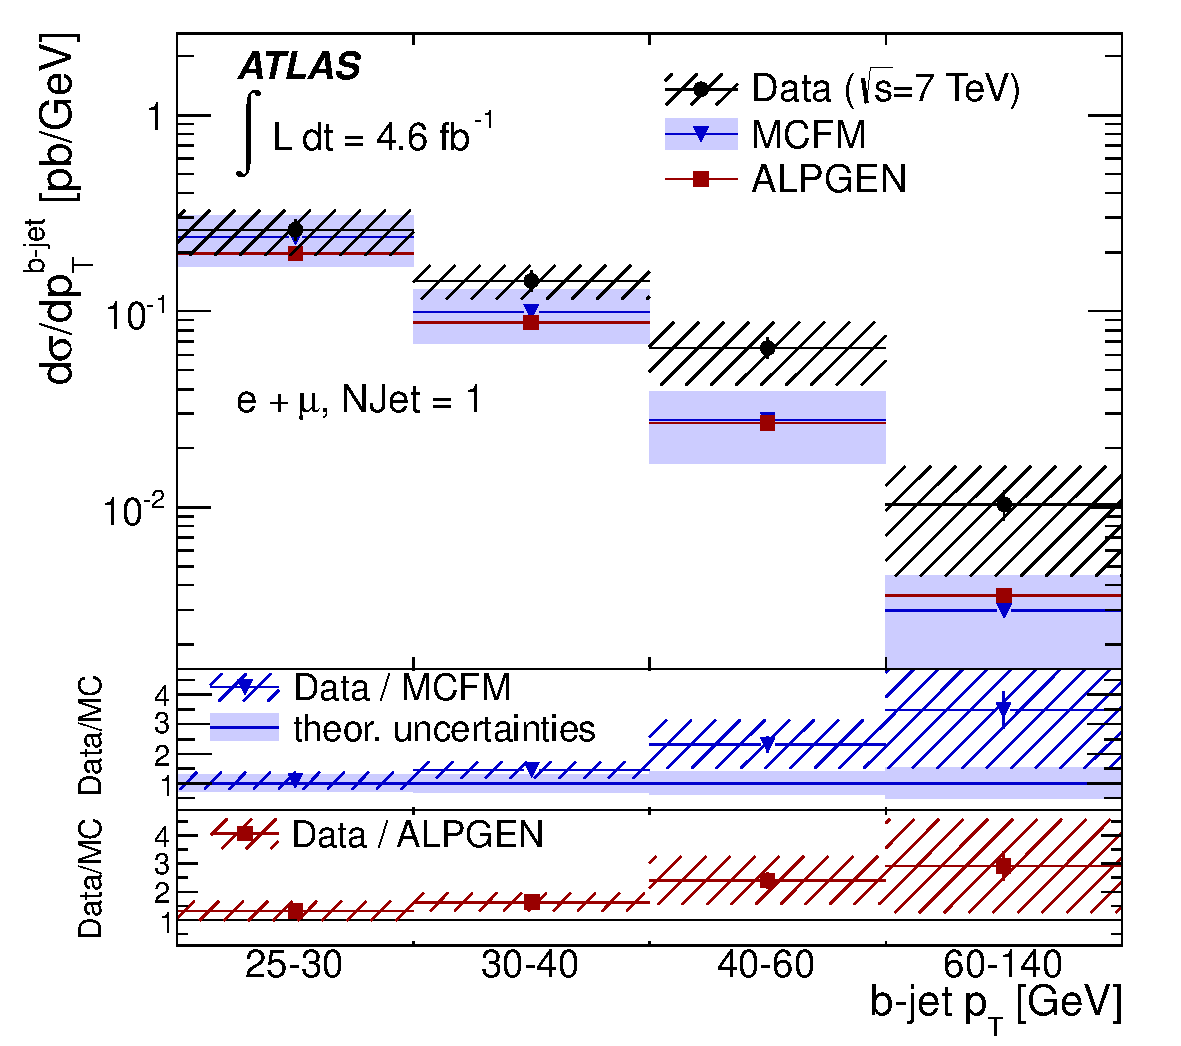
\includegraphics[width=0.48\textwidth]{fig_08a.pdf}
	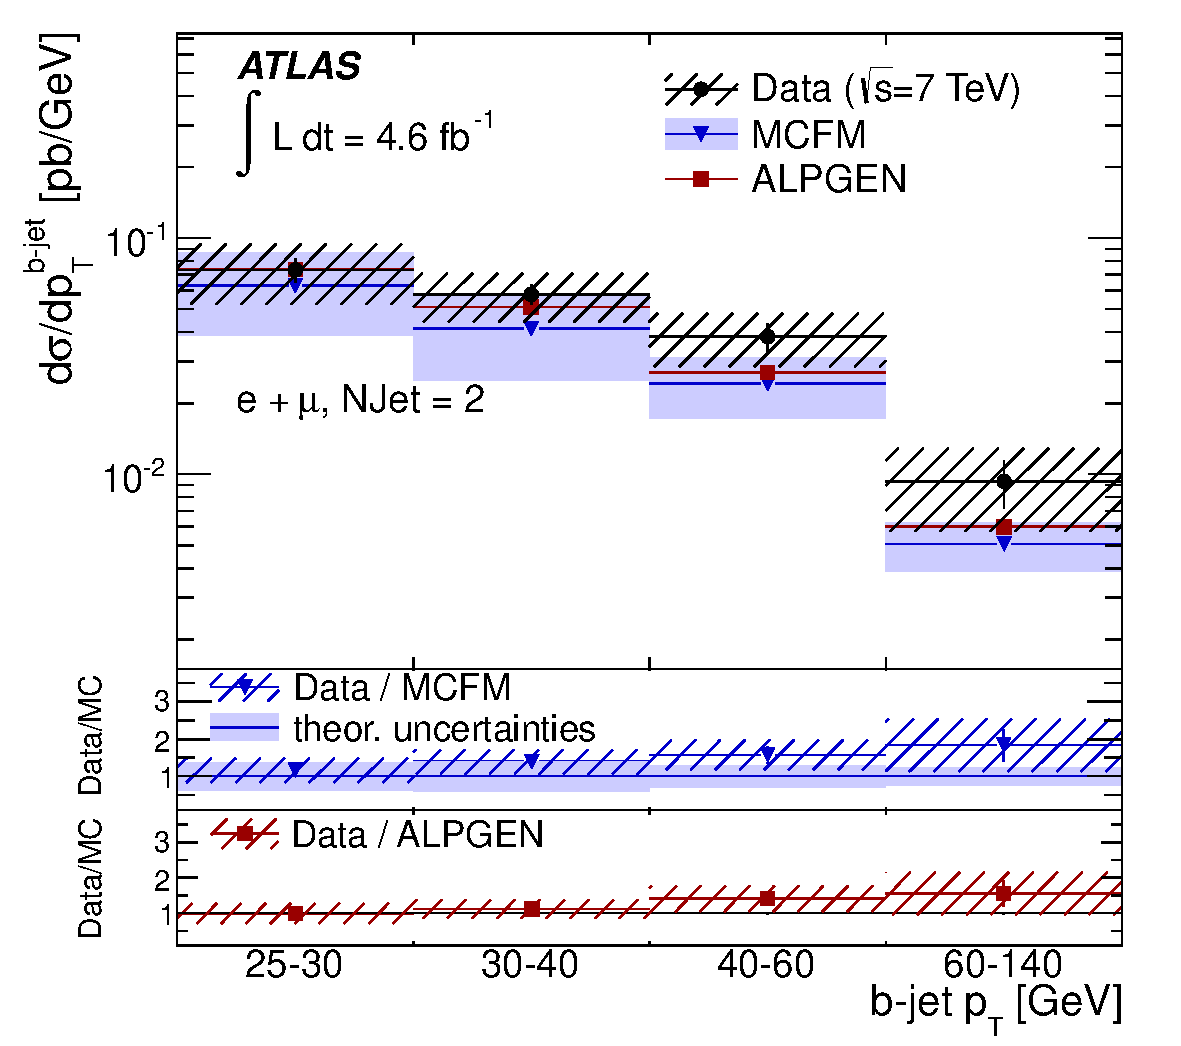
\includegraphics[width=0.48\textwidth]{fig_08b.pdf}
\caption{\label{fig:notop}
Measured differential $W+b$-jets cross-section after single-top subtraction as a function of the transverse momentum of the $b$-jet, in the case where the $b$-jet is the only jet in the fiducial region (left) or when there is an additional jet (right). 
%The cross sections are obtained by combining the electron and muon channels. 
The measurements are compared to the a calculation of $W+b$-jet production in the absence of top quark propagators obtained using ALPGEN interfaced to HERWIG and JIMMY and scaled by a NNLO inclusive $W$ normalization factor, and ACERMC interfaced to PYTHIA and scaled to a NLO single-top cross-section. 
The ratios between measured and predicted cross-sections are also shown. From~\protect\cite{Aad:2013vka}.}
\end{figure}

Several things may be noted:
\begin{itemize}
\item In neither case does the theory describe the data especially well. This is a challenging
final state to predict and the theory is likely to be superseded by more sophisticated and 
accurate predictions in future (indeed, NLO implementations of this
process in MC are already available, as discussed in
Section~\ref{thisLH_Vbb} of these proceedings). This strongly mitigates against embedding in a dependency 
on the theory in the experimental analysis - as is the case if the background is subtracted at detector-level - 
and is a strong motivation for the unsubtracted version of the
measurement. 
\item The contributions from diagrams with and without top are comparable (compare the cross section in the highest $p_T$ bin, 
for example).
\item The data uncertainties on the unsubtracted version are smaller.
\end{itemize}

Integrated over $p_T$, the unsubstracted fiducial cross section is
$9.6 \pm 0.2 (stat) \pm 1.7 (syst)$ pb, a fractional systematic uncertainty of 18\%.
The corresponding subtracted measurement is 
$7.1 \pm 0.5 (stat) \pm 1.4 (syst)$ pb, a fractional systematic uncertainty of 20\%
- a small but noticeable decrease in precision. Looking in more detail, the main contributions 
to the systematic errors are
\begin{itemize}
\item Jet energy scale: 10-50\%
\item Modelling of initial and final state QCD radiation on these two processes and on $t\bar{t}$: 2-30\%
\item $b$-tagging: 1-8\%
\item MC modelling (but only of the $Wb$ “signal”): 2-8\%
\end{itemize}
The fact that jet energy scale dominates masks, to a large extent, the effect of the modelling uncertainties introduced by
the background subtraction.
The uncertainty due to the modelling of QCD radiation varies strongly with jet $p_T$. 
This is exactly the kind of model dependence which one would expect to increase if a theory-based background
subtraction is made, and indeed, in the highest $p_T$ bin the systematic uncertainty goes from 16\% before subtraction 
to 54\% after it. (Compare Table~4 with Table~9 of Ref.\cite{Aad:2013vka}.) 

The comparisons were repeated using Sherpa 2.2~\cite{Gleisberg:2008ta} and Herwig7~\cite{Bellm:2015jjp}. 

For Sherpa, all intermediate particles in the matrix element are kept on-shell and the AMEGIC 
ME generator is used for LO calculations~\cite{Krauss:2001iv}. Only decays of the $W$ boson to the 
electron channel are allowed. Multi-parton interactions are switched off. 
The Sherpa default 5-flavour pdf library (NNPDF~\cite{Ball:2014uwa}) is used. In $Wb$ production
without tops, the $b$-quark is treated as massive with a mass of
4.75~GeV and the $W$ boson is treated through the narrow width approximation. The order of the electroweak couplings is fixed to 2. 
For single top production, the $b$-quark is treated as massless in the matrix element calculation
but retains its mass settings in the rest of the simulation. QCD and EW order couplings are not
fixed. Production modes include all channels: $s$-channel, $t$-channel and $tW$ single-top channels.

For Herwig, the built-in matrix elements for $W$+jet and single top were used. All leptonic decays
were generated, but the electron only channel was selected in Rivet, with a normalisation factor
of three applied post-hoc. Production includes $s$-channel,
$t$-channel and $tW$ single-top channels. The pdf MMHT2014~LO~\cite{Harland-Lang:2014zoa} is used. 

The comparison of the non-top diagrams only to the subtracted data is shown in Fig~\ref{fig:subtracted}. 
With these settings, Herwig gets the normalisation correct, agrees with the data normalisation and with
the shape of the 1-($b$)-jet contribution, but fails to describe the $p_T$ dependence of the 2-jet contribution.
Sherpa models the $p_T$ dependence of both contributions well, but overshoots the normalisation of the 1-jet
contribution by nearly a factor of 2.

\begin{figure}
\centering
	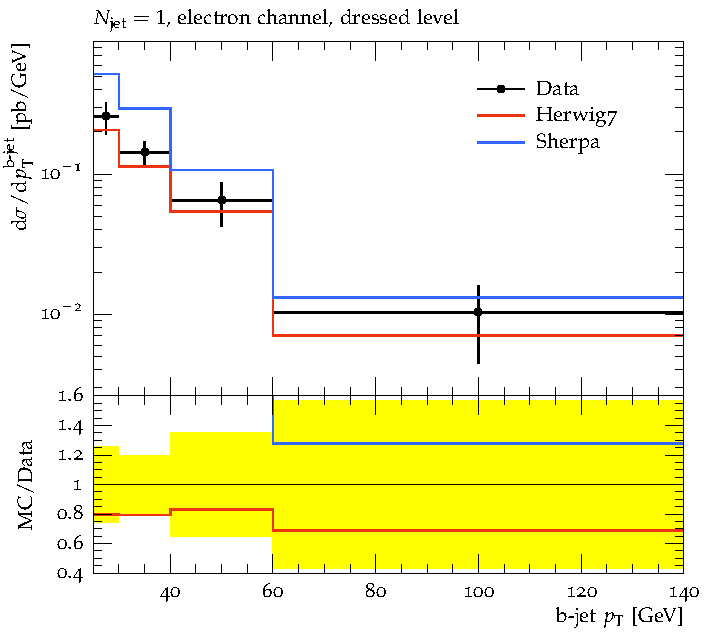
\includegraphics[width=0.48\textwidth]{subtracted_h7_s22-1jet.pdf}
	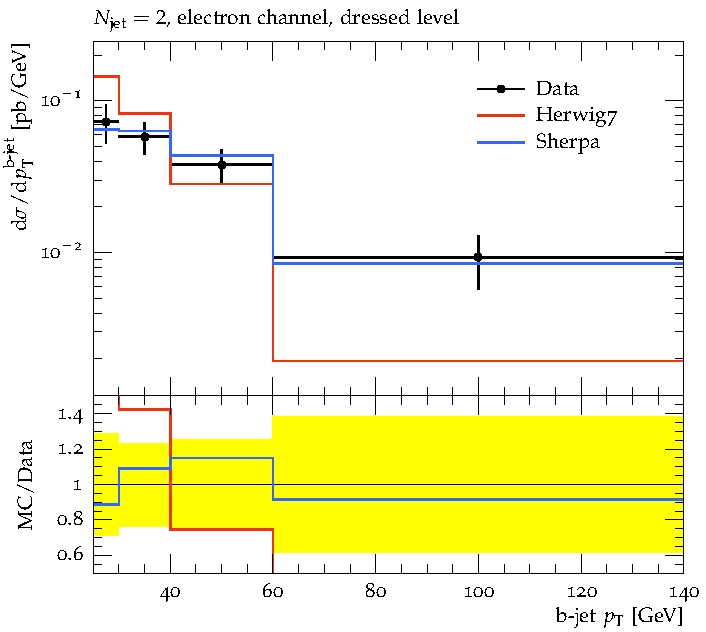
\includegraphics[width=0.48\textwidth]{subtracted_h7_s22-2jet.pdf}
\caption{\label{fig:subtracted}
  Measured differential $W+b$-jets cross-section after single-top subtraction as a function of the
  transverse momentum of the $b$-jet, in the case where the $b$-jet is the only jet in the fiducial region
  (left) or when there is an additional jet (right). The measurements are compared to the expectations of
  Sherpa and Herwig, for $Wb$ production processes excluding diagrams containing top quarks.}
\end{figure}

In Figs~\ref{fig:unsubtracted} the unsubtracted measurement is shown, compared to Herwig and Sherpa.
The contribution from non-top diagrams is shown again, as well as sum of this and the single top
contributions expected by the generator. (Interference terms are neglected.) Herwig again gets the
normalisation about right, and models the $p_T$ distribution of the 1-jet distribution well, while
struggling with this dependences for the 2-jet distribution. Sherpa still overshoots normalisation of
the 1-jet contribution (this time by about 65\%), but models the normalisation of the 2-jet contribution,
and the $p_T$ dependence of both contributions, reasonably well within the data uncertainties.

\begin{figure}
\centering
	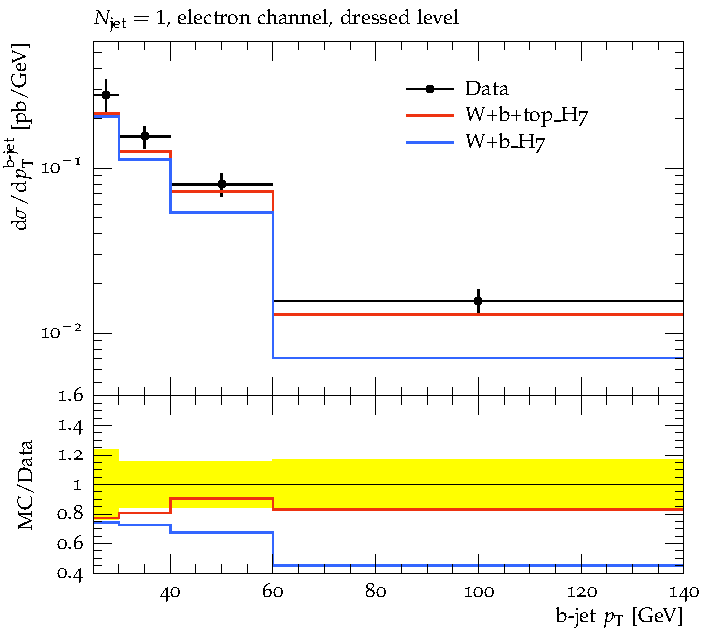
\includegraphics[width=0.48\textwidth]{unsubtracted-h7-1jet.pdf}
	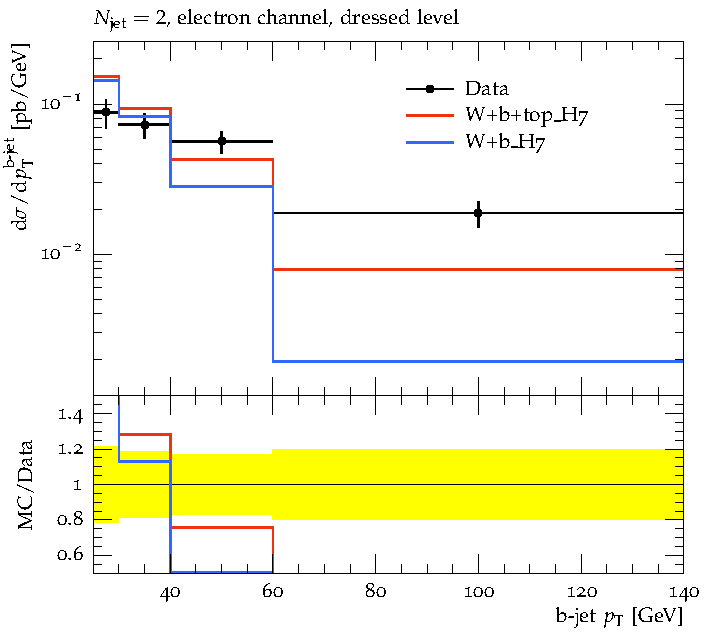
\includegraphics[width=0.48\textwidth]{unsubtracted-h7-2jet.pdf}
	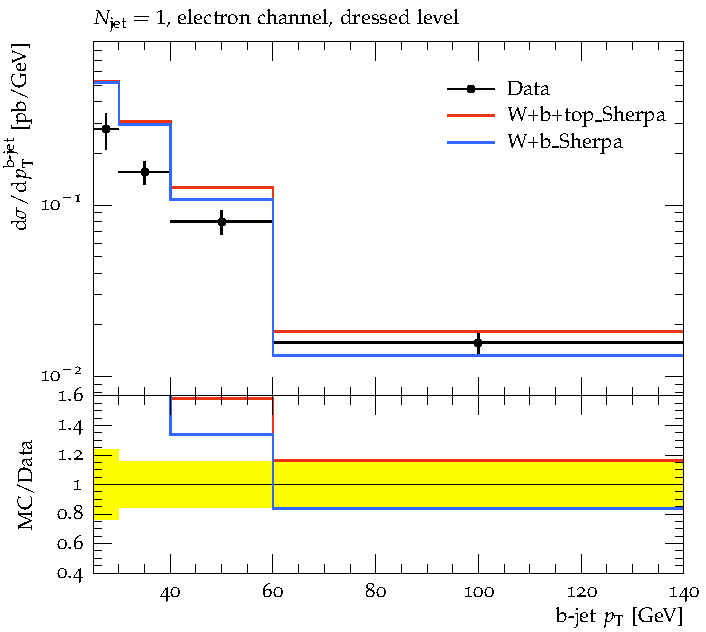
\includegraphics[width=0.48\textwidth]{unsubtracted-s22-1jet.pdf}
	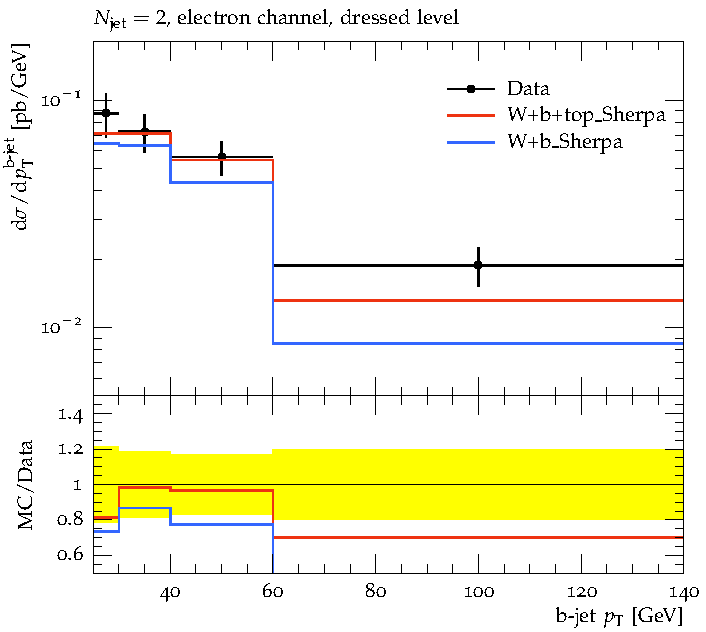
\includegraphics[width=0.48\textwidth]{unsubtracted-s22-2jet.pdf}
\caption{\label{fig:unsubtracted}
  Measured differential $W+b$-jets cross-section, including single-top contributions, as a function of the
  transverse momentum of the $b$-jet, in the case where the $b$-jet is the only jet in the fiducial region
  (left) or when there is an additional jet (right).  The measurements
  are compared to the Sherpa (top) and Herwig (bottom)
  calculations of $W+b$-jet production including resonant top contributions, but excluding finite width effects
  and interference terms between top and non-top diagrams. The contribution from non-top diagrams alone is
  also shown.}
\end{figure}

In Fig.~\ref{fig:13tev} we show the MC predictions for 13~TeV collisions. These measurements have yet to be
performed, but the main point to be made here is that the total top contribution rises from 15\% (32\%)
to 23\% (42\%) according to Sherpa (Herwig), with greater effects in some regions.  This shows that any
problems and uncertainties associated with the subtraction of irreducible backgrounds are likely to become
more severe at higher energies. The differences between the generators themselves is another indication of the 
challenges associated with predicting these cross sections, and thus the need to minimise the theory
dependence of the measurement.
  
\begin{figure}
\centering
	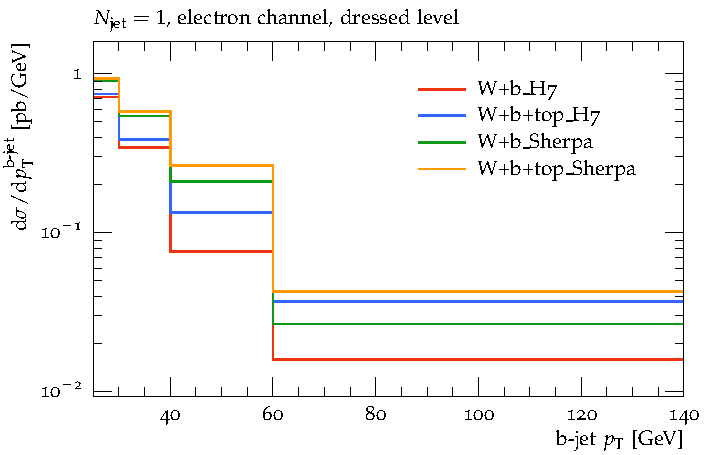
\includegraphics[width=0.48\textwidth]{13tev-1jet.pdf}
	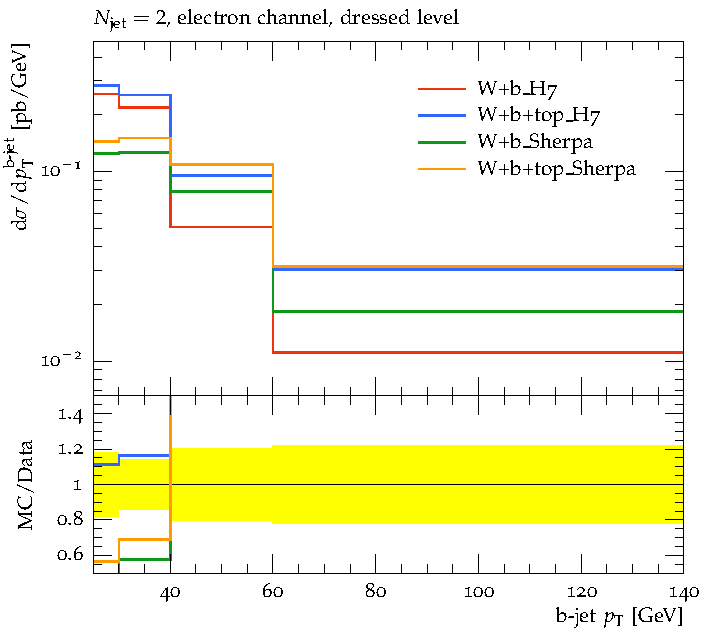
\includegraphics[width=0.48\textwidth]{13tev-2jet.pdf}
\caption{\label{fig:13tev}
  Differential $W+b$-jets cross-section at 13 TeV as a function of the
  transverse momentum of the $b$-jet, in the case where the $b$-jet is the only jet in the fiducial region
  (left) or when there is an additional jet (right). In both Sherpa and Herwig
  calculations of $W+b$-jet production including resonant top contributions, finite width effects 
  and interference terms between top and non-top diagrams are not
  taken into account. The contributions from non-top diagrams alone are also shown.}
\end{figure}

\subsection{Diboson plus jet production}

Processes in which two $W$-bosons and two jets (including possibly $b$-jets) are produced are of great interest
at the LHC.  Contributing amplitudes include
\begin{itemize}
\item $t\bar{t}$ (with on- or off-shell top quarks),
\item genuine QCD processes with $b$ quarks already entering from the initial state or being
  pair-produced in the final state through gluon splitting amplitudes, 
\end{itemize}
and, to a lesser extent,
\begin{itemize}
\item electroweak processes such as vector-boson fusion diagrams including the Higgs boson
  as a propagator and $b$-associated Higgs boson production.
\end{itemize}
In Sherpa, the leading order processes for $t\bar{t}$ and $tWb$ (both with on-shell tops), and $WWb\bar{b}$
(excluding all top contributions) were generated separately, and the full leading order $WWb\bar{b}$ process,
including all top contributions was also generated for comparison. All processes were generated for centre-of-mass
energies of 13~TeV. 

An initial set of basic selection cut was applied, requiring two isolated leptons with $|\eta| < 2.5, p_T > 25$~GeV and
missing $E_T > 25$~GeV, typical of an experimental analysis. The multiplicity of jets (identified with the anti-$k_T$
algorithm, $R=0.4$, $p_T > 25$~GeV, $|\eta| < 4.5$) in events passing these cuts is shown in Fig.~\ref{fig:wbf_before}.
It can be seen that the diagrams involving at least one top quark dominate, though the contribution of non-top diagrams
is significant at low jet multiplicities.  Fig.~\ref{fig:wbf_before} also compares the incoherent sum of the different
contributions with the coherently generated $WWb\bar{b}$ process. It can be seen that the interference terms are largely
positive.
%I've commented this out: I am not sure if we actually see negative interference or statistics here
% though they become negative for jet multiplicities above four.  

Further cuts were applied to mimic a vector-boson-fusion like analysis, requiring that there are at least two jets in
opposite hemispheres of rapidity, with a rapidity difference between them
$\Delta y_{jj} > 2.4$ and a dijet invariant
mass $m_{jj}>500$~GeV, and after additional cuts on the transverse mass
of the dilepton $m_{\ell\ell} > 20$~GeV and missing $E_T > 40$~GeV.
Fig.~\ref{fig:wbf_after} shows that the same general features persist, with the interference terms being large and
positive for jet mulitiplicities below five.

\begin{figure}
\centering
	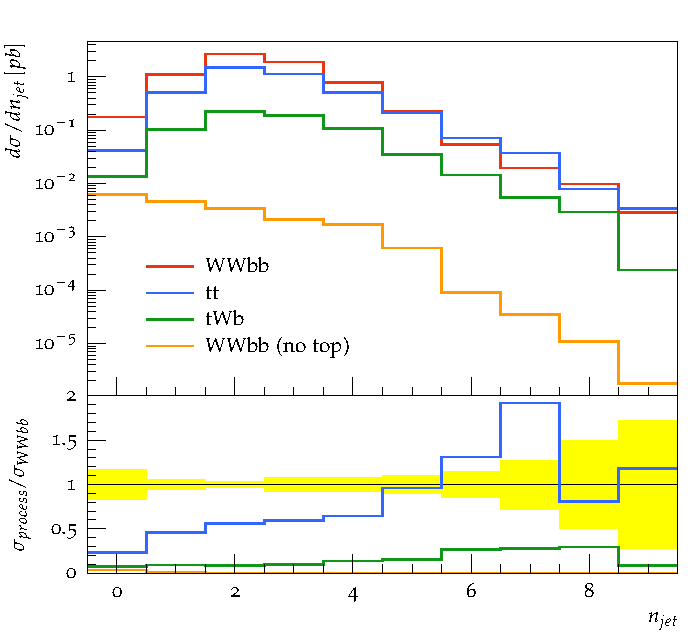
\includegraphics[width=0.48\textwidth]{WBF_njets_before_contribs.pdf}
	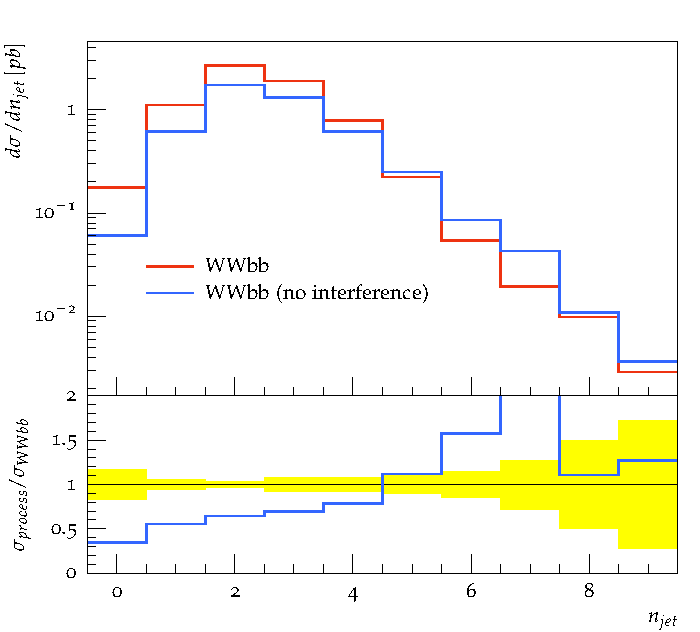
\includegraphics[width=0.48\textwidth]{WBF_njets_before.pdf}
\caption{\label{fig:wbf_before}
  13 TeV $WWb\bar{b}$ events simulated using Sherpa.
  (left) individual contributions (right) comparison between incoherent and coherent sums.}
\end{figure}

\begin{figure}
\centering
	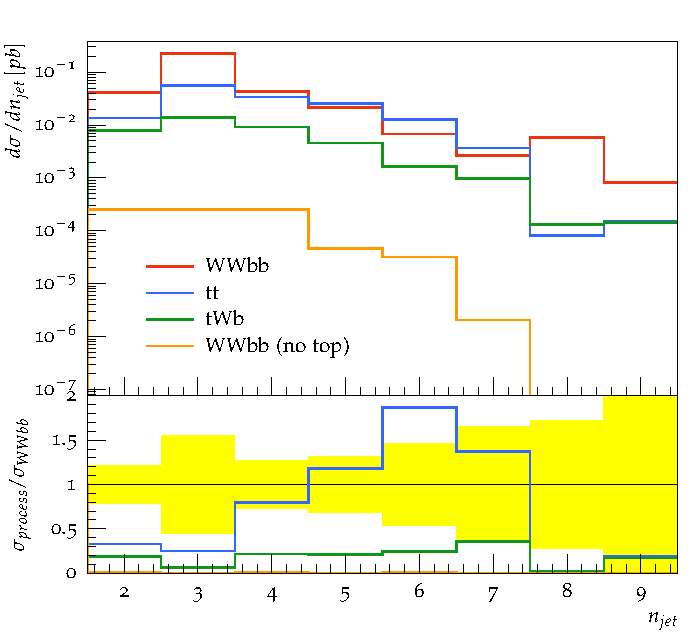
\includegraphics[width=0.48\textwidth]{WBF_njets_after_contribs.pdf}
	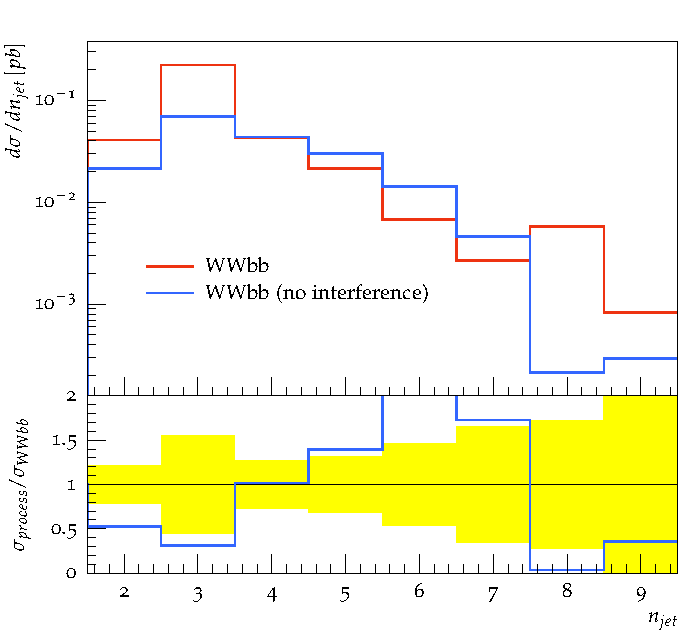
\includegraphics[width=0.48\textwidth]{WBF_njets_after.pdf}
\caption{\label{fig:wbf_after}
  13 TeV $WWb\bar{b}$ events simulated using Sherpa, after vector-boson-fusion selection cuts. 
  (left) individual contributions (right) comparison between incoherent and coherent sums.}
\end{figure}

\subsection{Conclusions}\label{sec:conclusions}

This brief study exploits a measurement made by ATLAS, and the multi-process capabilities of Sherpa,
to illustrate the fact that many apparently distinct processes may contribute to the same measurable
final state. The treatement of the these processes by the experiments is important. Subtraction of
irreducible backgrounds can increase the model-dependence of systematic uncertainties, and is
unphysical, in the sense that interference terms are not treated correctly. In this discussion,
both these effects are observed.  The 7~TeV $Wb$ measurement by ATLAS shows increased systematic
uncertainties in the region of high jet-$p_T$ if top contributions are subtracted.  These
contributions will become more significant at 13~TeV, and so the problem can be expected to become
worse. And Sherpa studies indicate that, even after realistic selection of vector-boson-fusion-like
toplogies, interference terms are signficant in $WWbb$ production.  In conclusion, the treatment of
irreducible background in future measurements at the LHC merits more careful attention.

\bibliography{backsub}

\end{document}


